% Tutto quello riguardante il progetto andrà in questo capitolo 

\chapter{Tecnologie utilizzate}\label{chap:tec}
\section{Ambiente di sviluppo}
\subsection{Docker}
	\begin{figure}[H] 
		\centering
		
\includegraphics[scale=0.3]{docker}
		\caption{Logo Docker}
	\end{figure}
Docker permette di automatizzare lo sviluppo di applicazione dentro a 
determinati container software, 
in modo da fornire una virtualizzazione a livello del sistema operativo Linux
senza che sia necessario istanziare delle macchine virtuali pienamente 
operative.
I container sono assimilabili a delle macchine virtuali modulari che hanno il 
pregio di essere molto 
leggere: in questo modo risulta più facile  creare, distribuire, copiare e spostare 
i container da un 
ambiente all'altro.
Ogni container è un processo isolato dagli altri container e dal sistema ospite stesso:  ogni volta che 
viene mandato in esecuzione si avrà un ambiente pulito, con le caratteristiche desiderate. \\
Per sviluppare l'applicazione Teamwork è stato utilizato Docker 18.03 Community Edition per Ubuntu 
Bionic. In questo modo si è potuto caricare nelle macchine locali un container di Zimbra e del core 
Zextras con la zimlet OpenChat caricata così da sviluppare l'applicativo in un ambiente sicuro e pulito.

\subsection{IntelliJ IDEA} \label{subsec:IntelliJ}
	\begin{figure}[H] 
		\centering
		
\includegraphics[scale=0.2]{intellij-idea}
		\caption{Logo IntelliJ IDEA}
	\end{figure}
IntelliJ IDEA è un Integrated Development Environment (IDE) multi-linguaggio e 
multi-piattaforma. 
È stata utilizzata la versione Ultimate in quanto era necessario un editor che 
supportasse  
JavaScript/TypeScript, mentre la Community version non supporta questi 
linguaggi. 
Dovendo creare un'applicazione con numerose referenze al codice della zimlet 
OpenChat e di Zimbra 
sono state sfruttate al meglio le funzionalità per analizzare il codice e 
comprendere le 
dipendenze esistenti.

\subsection{Expo} \label{subsec:expo}
	\begin{figure}[H] 
		\centering
		
\includegraphics[scale=0.05]{expo}
		\caption{Logo Expo}
	\end{figure}
Expo è una toolchain open source che permette la gestione di un progetto React 
Native utilizzando l'SDK di Expo. L'SDK Expo è una libreria nativa e JavaScript 
che fornisce l'accesso alle funzionalità del sistema del dispositivo (come la 
fotocamera, i contatti, la memoria locale) senza il bisogno di utilizzare xCode 
o Android Studio, né di utilizzare codice nativo. Fornisce l'accesso a servizi 
che in genere sono difficili da gestire nativamente, ma sono richiesti da quasi 
tutte le app come le notifiche push o creare binari nativi pronti per la 
distribuzione nell'app store.
Inoltre risulta molto facile lo sviluppo e il test dato che permette delle 
build automatiche nei loro server che possono eseguire in real-time il codice 
sia in simulatori che in dispositivi mobili.


\section{Linguaggi, librerie e strumenti di programmazione}

\subsection{React Native}
\begin{figure}[H] 
	\centering
	
\includegraphics[scale=0.1]{React}
	\caption{Logo React Native}
\end{figure}
React Native è un framework per lo sviluppo di applicazioni mobile in
JavaScript, destinate a piattaforme native. Questo permette di 
unificare l'esperienza di sviluppo su diversi sistemi operativi. Infatti React 
Native utilizza gli stessi blocchi fondamentali dell'interfaccia utente che 
vengono utilizzate da app native iOS e Android che utilizzano invece i 
linguaggi Swift e Java.
Si possono comunque integrare dei componenti scritti in Objective-C, 
Java o Swift così da passare al codice nativo nel caso fosse necessario 
ottimizzare alcuni aspetti dell'applicazione in base alla piattaforma. 
React Native si basa su ReactJS dove appare fondamentale il concetto di 
componente. Un componente è qualcosa che ha uno stato, che può accettare 
delle proprietà e che ha un proprio ciclo di vita. Questo approccio di 
sviluppo atomico risulta perfetto per effettuare Unit Test o per creare 
componenti più complessi includendone altri più semplici.

\subsection{TypeScript}
\begin{figure}[H] 
	\centering
	
\includegraphics[scale=0.07]{ts}
	\caption{Logo TypeScript}
\end{figure}
TypeScript è un linguaggio di programmazione sviluppato da Microsoft che 
estende la sintassi di JavaScript.  È nato per poter utilizzare le funzionalità di 
JavaScript per lo sviluppo di grandi applicazioni in quanto aumenta la 
sicurezza e la robustezza del codice tramite aggiunte come le classi, le 
interfacce, i moduli, la tipizzazione e altre funzionalità importanti per la 
comprensione di un grande progetto. 
TypeScript viene successivamente ricompilato in JavaScript per poter essere 
 interpretato da browser o app.

\subsection{TSLint}
\begin{figure}[H] 
	\centering
	
\includegraphics[scale=0.4]{TSlint}
	\caption{Logo TS Lint}
\end{figure}
TSLint è uno strumento di analisi statica per il codice scritto in TypeScript che offre funzionalità estendibili e personalizzabili per la leggibilità, la manutenibilità e gli errori di funzionalità. È supportato da molti dei moderni editor, compreso intelliJ IDEA (sez. \ref{subsec:IntelliJ}), utilizzato per il progetto.

\subsection{Redux}
\begin{figure}[H] 
	\centering
	
\includegraphics[scale=0.06]{redux}
	\caption{Logo Redux}
\end{figure}
Redux è una libreria Javascript per la gestione semplificata dello stato delle applicazioni web. Tramite ReactJS e React Native ogni componente possiede uno stato che può cambiare durante il suo ciclo di vita. Questo stato è interno ad ogni singola componente ed è difficile, a volte impossibile, la comunicazione di questi dati tra componenti diverse. 
Tramite Redux, invece, si può creare uno store condiviso contenente dei dati che verranno utilizzati da ogni componente in cui ogni modifica verrà sincronizzata per mantenere i dati coerenti tra le varie componenti.
Redux è stato implementato basandosi su una particolare architattura: Flux.

\subsubsection{Flux}
 Flux è un pattern architetturale che ha ispirato Redux, utilizzato per la creazione di applicazioni web lato client. Esso utilizza un flusso di dati unidirezionale per gestire al meglio la sincronizzazione degli stati tra le componenti React. In questo modo si è sicuri che lo stato dello store sia sempre uguale in tutte le componenti che compongono la view.
 \begin{figure}[H] 
 	\centering
 	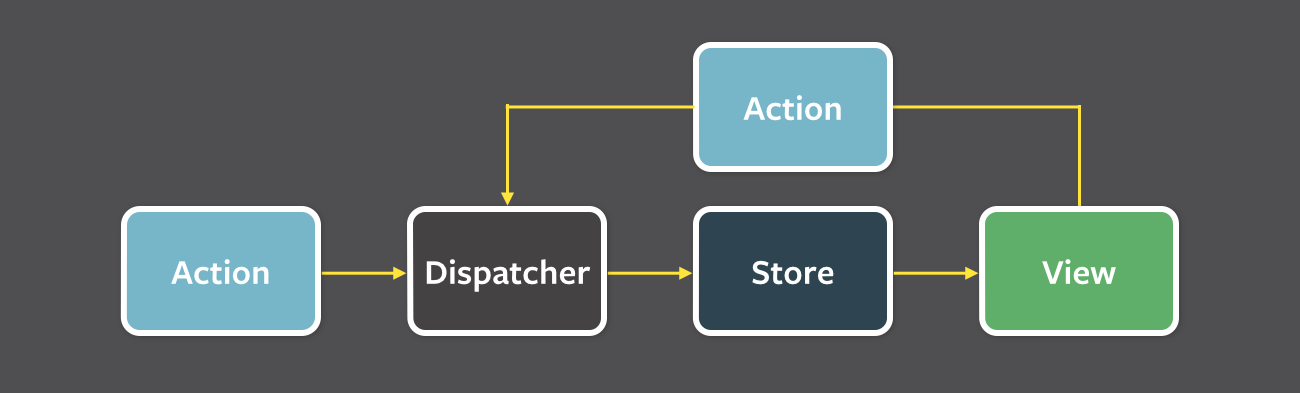
\includegraphics[scale=0.3]{flux}
 	\caption{Flusso dei dati in Flux}
 \end{figure}
 Le view, però, possono causare delle action che modificano lo stato dello store ma esso sarà interamente propagato in tutto il sistema così da evitare inconsistenza dei dati nelle view.
 
\section{Strumenti di verifica e valutazione}

\subsection{Genymotion}
\begin{figure}[H] 
	\centering
	
\includegraphics[scale=0.2]{genymotion2}
	\caption{Logo Genymotion}
\end{figure}
Genymotion è un emulatore software di dispositivi Android. Si integra perfettamente con Expo(sez. \ref{subsec:expo}), utilizzato per la gestione di questo progetto, permettendo di avere un riscontro dell'app in real-time durante lo sviluppo e di verificare e testare l'applicazione su più device. Emula più di 3000 configurazioni virtuali di dispositivi Android (tra versioni, dimensioni schermo, capacità hardware, ecc..). 

\subsection{React Native Debugger}
\begin{figure}[H] 
	\centering
	
\includegraphics[scale=0.15]{react-native-debugger}
	\caption{Logo React Native Debugger}
\end{figure}
React Native Debugger è un applicazione standalone per il debug di app in React Native. Si basa sul remote bedugger disponibile quando si monitora un progetto in un device fisico o virtuale.\\ Esso offre vari strumenti per il debug:
\begin{itemize}
	\item React Inspector, per ispezionare il layout e lo style di ogni componente dell'app;
	\item Redux DevTools, per monitorare gli store Redux utilizzati e le action svolte su di essi;
	\item Console, per visualizzare errori e avvisi che avvengono durante l'esecuzione del codice.
\end{itemize}

\subsection{Jest}
\begin{figure}[H] 
	\centering
	
\includegraphics[scale=0.13]{jest}
	\caption{Logo Jest}
\end{figure}
Jest è un framework di unit testing per JavaScript sviluppato ed utilizzato da Facebook per testare le proprie applicazioni in React. È una soluzione completa e pronta per la configurazione in quanto è automaticamente configurato quando si crea un progetto React Native.
Rispetto ad altri framework di unit testing offre dei vantaggi, come: 
\begin{itemize}
	\item vengono eseguiti solo i file di test relativi ai file modificati;
	\item gestisce automaticamente le dipendenze durante l'esecuzione dei test;
	\item permette di testare in modo sincroni il codice asincrono;
	\item esegue i test in processi paralleli così che finiscano prima.
\end{itemize}
Inoltre Jest funziona con qualsiasi linguaggio compile-to-JavaScript. Sia il codice da testare che i test stessi possono essere scritti in TypeScript, linguaggio utilizzato per questo progetto. 
